% Editorial prototype only. Exact states/actions/ranks from c24 figures/cell_paths.tex.
% Not included in c24, not a new experiment or proof.
\begin{figure}[!htbp]
\centering
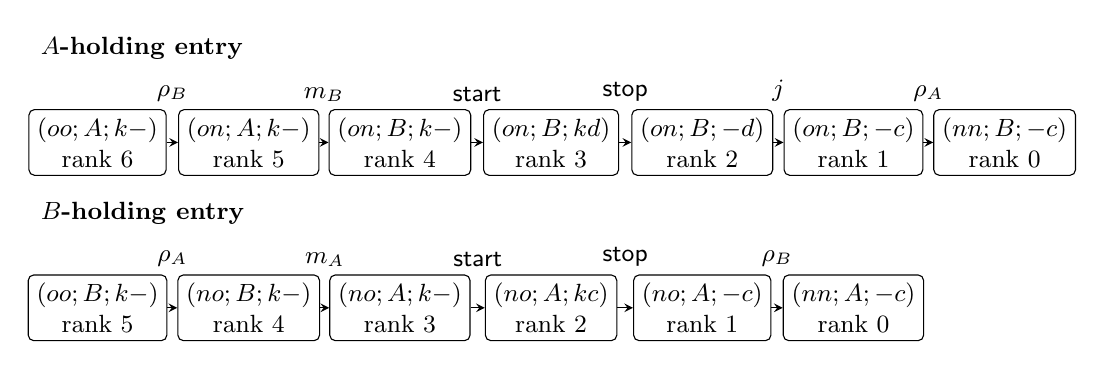
\begin{tikzpicture}[x=1.92cm,y=1cm,
  state/.style={draw,rounded corners=2pt,inner sep=3pt,font=\small,align=center},
  edge/.style={->,>=stealth},
  action/.style={font=\small,above,yshift=4mm}]
\node[anchor=west,font=\small\bfseries] at (-.44,1.2) {$A$-holding entry};
\node[state] (a0) at (0,0) {$(oo;A;k{-})$\\rank 6};
\node[state] (a1) at (1,0) {$(on;A;k{-})$\\rank 5};
\node[state] (a2) at (2,0) {$(on;B;k{-})$\\rank 4};
\node[state] (a3) at (3,0) {$(on;B;kd)$\\rank 3};
\node[state] (a4) at (4,0) {$(on;B;{-}d)$\\rank 2};
\node[state] (a5) at (5,0) {$(on;B;{-}c)$\\rank 1};
\node[state] (a6) at (6,0) {$(nn;B;{-}c)$\\rank 0};
\draw[edge] (a0)--node[action]{$\rho_B$}(a1);
\draw[edge] (a1)--node[action]{$m_B$}(a2);
\draw[edge] (a2)--node[action]{$\mathsf{start}$}(a3);
\draw[edge] (a3)--node[action]{$\mathsf{stop}$}(a4);
\draw[edge] (a4)--node[action]{$j$}(a5);
\draw[edge] (a5)--node[action]{$\rho_A$}(a6);
\node[anchor=west,font=\small\bfseries] at (-.44,-.9) {$B$-holding entry};
\node[state] (b0) at (0,-2.1) {$(oo;B;k{-})$\\rank 5};
\node[state] (b1) at (1,-2.1) {$(no;B;k{-})$\\rank 4};
\node[state] (b2) at (2,-2.1) {$(no;A;k{-})$\\rank 3};
\node[state] (b3) at (3,-2.1) {$(no;A;kc)$\\rank 2};
\node[state] (b4) at (4,-2.1) {$(no;A;{-}c)$\\rank 1};
\node[state] (b5) at (5,-2.1) {$(nn;A;{-}c)$\\rank 0};
\draw[edge] (b0)--node[action]{$\rho_A$}(b1);
\draw[edge] (b1)--node[action]{$m_A$}(b2);
\draw[edge] (b2)--node[action]{$\mathsf{start}$}(b3);
\draw[edge] (b3)--node[action]{$\mathsf{stop}$}(b4);
\draw[edge] (b4)--node[action]{$\rho_B$}(b5);
\end{tikzpicture}
\caption{One policy from both entries. States list versions of $A,B$, the workpiece holder, and old/new monitors; the holder also determines the interval monitor. A dash means inactive. Every edge decreases the remaining-step rank. The two rank-zero states match the respective fixed-controller targets.}
\label{fig:cell-paths}
\end{figure}
